\documentclass{paper}

%\usepackage{times}
\usepackage{epsfig}
\usepackage{graphicx}
\usepackage{amsmath}
\usepackage{amssymb}
\usepackage{color}
\usepackage{caption}
\usepackage{subcaption}


% load package with ``framed'' and ``numbered'' option.
%\usepackage[framed,numbered,autolinebreaks,useliterate]{mcode}

% something NOT relevant to the usage of the package.
\setlength{\parindent}{0pt}
\setlength{\parskip}{18pt}
\graphicspath{{images/}}


\usepackage[latin1]{inputenc} 
\usepackage[T1]{fontenc} 


\usepackage{listings} 
\lstset{% 
   language=Matlab, 
   basicstyle=\small\ttfamily, 
} 



\title{Assignment 1}



\author{Jenni Simon\\09-116-005}
% //////////////////////////////////////////////////


\begin{document}



\maketitle


% Add figures:
%\begin{figure}[t]
%%\begin{center}
%\quad\quad   \includegraphics[width=1\linewidth]{ass2}
%%\end{center}
%
%\label{fig:performance}
%\end{figure}

\section*{Photometric Stereo}



\paragraph{1. Calibration}
\subparagraph{Algorithm}
Let $r$ be the radius and $c=(c_x,c_y)$ be the image-coordinates of the
sphere. Further let $s_i=(s_{ix},s_{iy})$ be the image-coordinates of the
highlights on the sphere in image $i$ for $i\in{\{1,\hdots,N\}}$. Let the
unit vector $d=(0,0,-1)$ denote the direction of the camera from any
point on the sphere. Both $r$ and $c$ can easily be inferred from the
provided object-masks and the spot-highlights $s_i $ can also easily be
located by looking for maximal intensity values in the images.

The 3D-coordinates of the surface-normal at a position $p=(p_{x},p_{y})$ on the sphere can then be computed as 
\begin{equation} 
\begin{split}
  n_x(p)  &=  \frac{p_x-c_x}{r}      \\
  n_y (p) &=  \frac{p_y-c_y}{r}      \\
  n_z(p)  &=  -\sqrt{1-n_x^2-n_y^2}   
\end{split}   
\end{equation}
Note that the normal $n(p)=(n_x,n_y,n_z)$ then already has unit length.
The unnormalised directions of the light-sources $L_i$ for $i\in{\{1,\hdots,N\}}$ are then given by 
\begin{equation} 
L_i=2\cdot (n(s_i))^Td\cdot n(s_i)-d
\end{equation}

\subparagraph{Resulting Light-Directions} 
Normalising these light-directions I obtained the following results
(row $i$ corresponds to $L_i^T$):
\begin{align}
\mathbf{L^T}= \left[ \begin{array}{ccc}
0.496 & -0.466 & -0.733\\
0.245 & -0.129 & -0.961 \\
-0.038 & -0.180 & -0.983 \\
-0.103 & -0.438 & -0.893 \\
-0.323 & -0.506 & -0.799 \\
-0.117 & -0.558 & -0.822 \\
0.287 & -0.418 & -0.862 \\
0.094 & -0.438 & -0.894 \\
0.209 & -0.342 & -0.916 \\
0.095 & -0.327 & -0.940 \\
0.129 & -0.046 & -0.990 \\
-0.136 & -0.359 & -0.923 
\end{array} \right] \nonumber
\end{align}


\paragraph{2. Computing Surface Normals and Grey Albedo}
\subparagraph{Algorithm} 
Let $I_i$ be a gray-level image and let $I_i(p)$ denote the intensity at
pixel $p$ for $i\in{\{1,\hdots,N\}}$. The pixel intensity can then be
modeled as $I_i(p)=\alpha(p)(n(p)^TL_i)$ (assuming diffuse objects and
distant point light sources). We can further combine the $I_i$'s into
a $M\times N$ matrix of image-intensities by vectorising the relevant
image pixels of image $I_i$. $M$ therefore stands for the number of
image pixels corresponding to the object and $N$ for the number of
images (and light-sources). Let $n$ denote the $3 \times M$ matrix of
the unknown surface normals.
The problem can then be written as $I=(\alpha n^T)L$, or
equivalently as $I^T=L^T(\alpha^T n)$ and we can
solve for the the unknown matrix $A=\alpha^T n$ via 
\begin{equation} 
A=(LL^T)^{-1}LI^T
\end{equation}
The matrix $(LL^T)^{-1}L$ is also called the pseudo-inverse of
$L$. From the definition $A=\alpha^T n$ we see that the albedo
$\alpha$ is given by the magnitude of the columns of $A$ and the
normals $n$ are given by the normalized columns of $A$. 

Having computed the normals, we can now solve for the individual red-,
green- and blue-albedo of the objects. To this end, let $I_r$ denote
the $M\times N$ matrix of vectorized red-channel images. Our model
again is $I_r=\alpha_r(n^TL)$, where $\alpha_r$ is the unknown
red-albedo. Let $G:=(n^TL)$. We solve for $\alpha_r$ by minimizing the error
\begin{equation} 
\alpha_r = \underset{\alpha} {\mathrm{argmin}} \Vert
I_r-\alpha_rG \Vert^2
\end{equation}
Taking derivatives and setting them to zero, we obtain the follow
formula for the albedo at pixel $p$:
\begin{equation} 
\alpha_r(p) = \frac{\sum_{i=1}^NG(p,i)\cdot I_r(p)}{\sum_{i=1}^NG(p,i)^2}
\end{equation}

\subparagraph{Results} 
Applying the above procedure to the dataset we obtain the gray albedos
in figure \ref{fig:GA} and the normal-maps shown in figure
\ref{fig:NM}. The normals in figure \ref{fig:NM} are visualized by
mapping the $x$-, $y$- and $z$-coordinates of the normals to
RGB-values in the range $1-255$.  Finally, figure \ref{fig:RGB} shows
the recovered color albedos.

\begin{figure*}[h!]
    \centering
    \begin{subfigure}[]{0.33\textwidth}
        \centering
        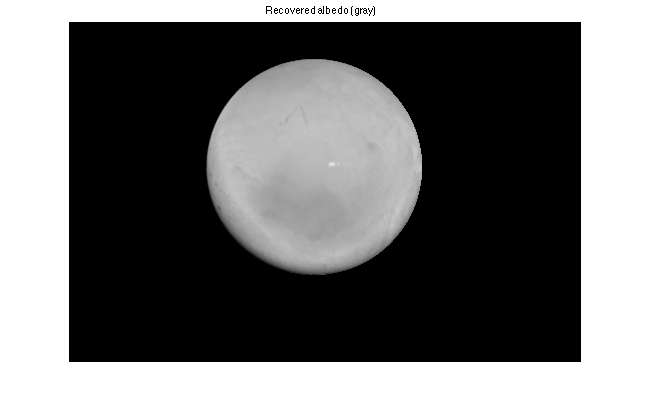
\includegraphics[height=1.2in]{sphereGA}
    \end{subfigure}%
    ~ 
    \begin{subfigure}[]{0.33\textwidth}
        \centering
        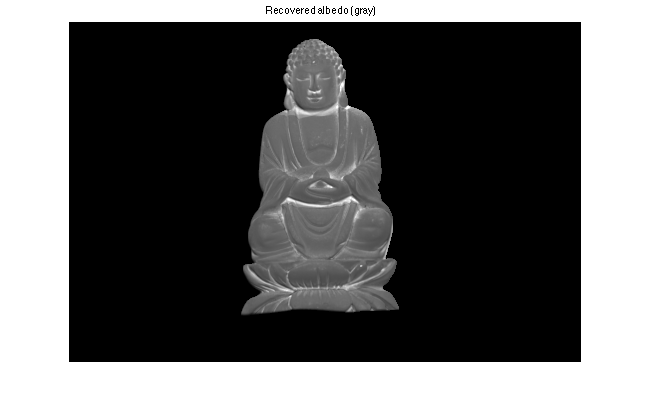
\includegraphics[height=1.2in]{buddhaGA}
    \end{subfigure}%
    ~ 
    \begin{subfigure}[]{0.33\textwidth}
        \centering
        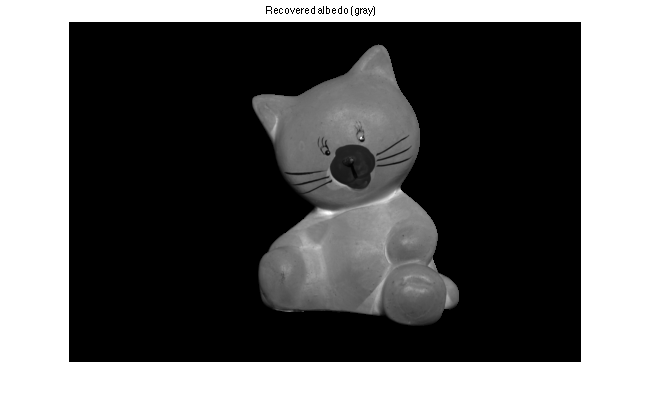
\includegraphics[height=1.2in]{catGA}
    \end{subfigure}
        \begin{subfigure}[]{0.33\textwidth}
        \centering
        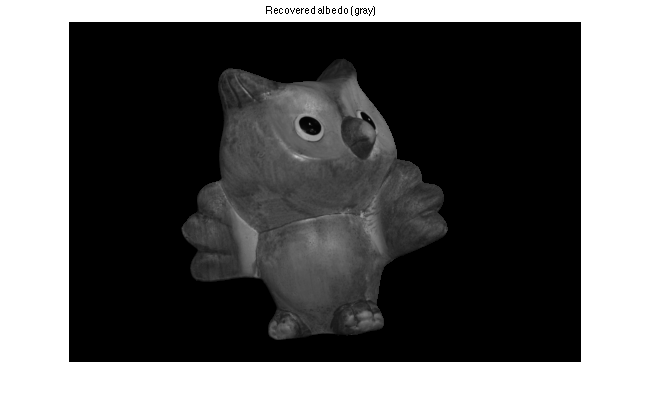
\includegraphics[height=1.2in]{owlGA}
    \end{subfigure}%
    ~ 
    \begin{subfigure}[]{0.33\textwidth}
        \centering
        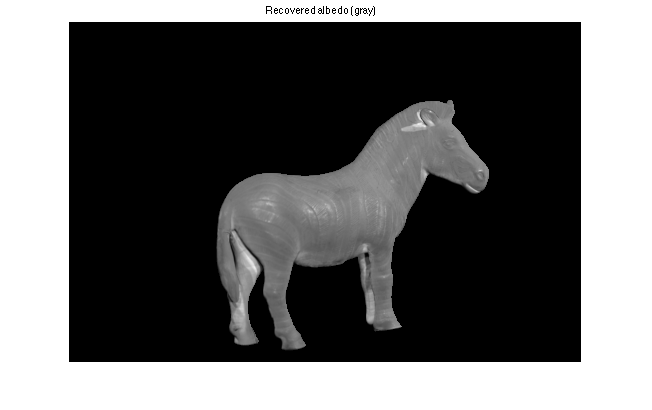
\includegraphics[height=1.2in]{zebraGA}
    \end{subfigure}%
    ~ 
    \begin{subfigure}[]{0.33\textwidth}
        \centering
        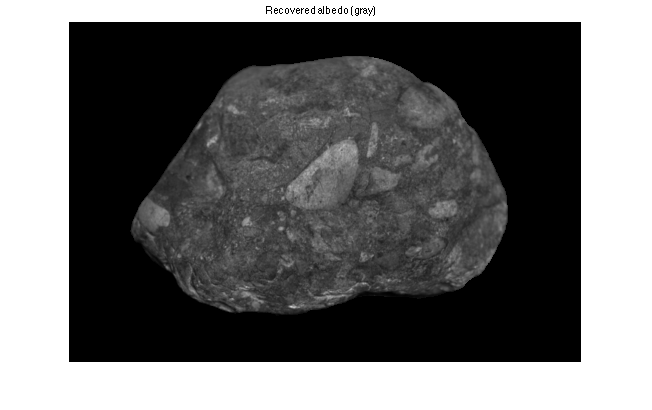
\includegraphics[height=1.2in]{rockGA}
    \end{subfigure}

    \caption{Recovered gray albedo}    
\label{fig:GA}

\end{figure*}

\begin{figure*}[h!]
    \centering
    \begin{subfigure}[]{0.33\textwidth}
        \centering
        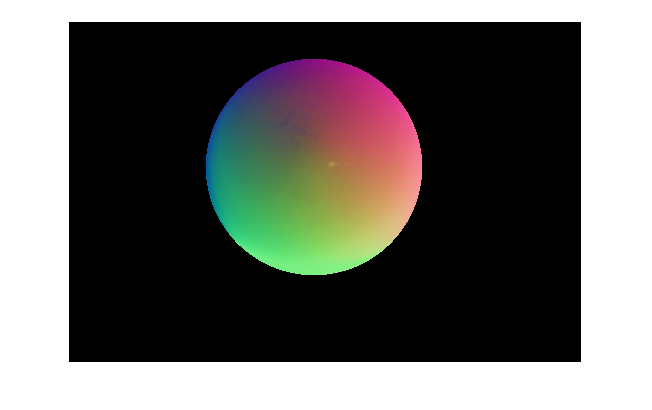
\includegraphics[height=1.2in]{sphereNM}
    \end{subfigure}%
    ~ 
    \begin{subfigure}[]{0.33\textwidth}
        \centering
        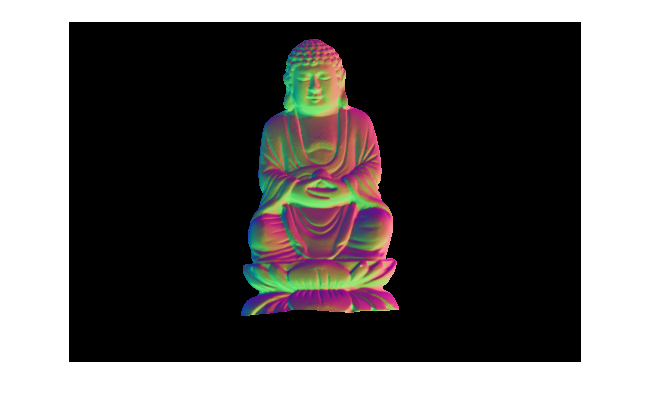
\includegraphics[height=1.2in]{buddhaNM}
    \end{subfigure}%
    ~ 
    \begin{subfigure}[]{0.33\textwidth}
        \centering
        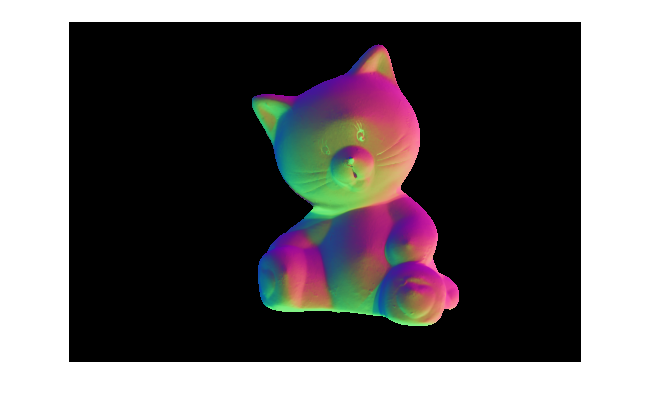
\includegraphics[height=1.2in]{catNM}
    \end{subfigure}
        \begin{subfigure}[]{0.33\textwidth}
        \centering
        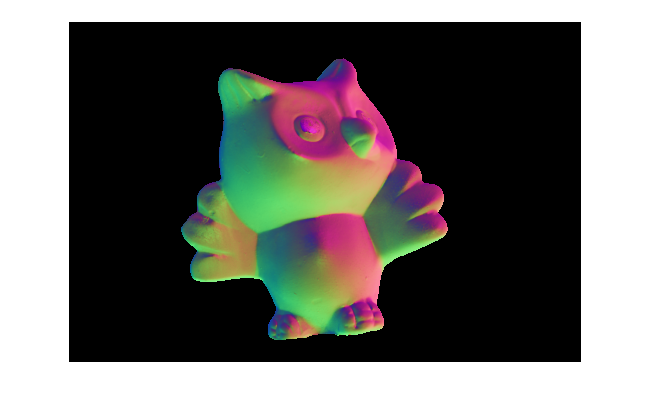
\includegraphics[height=1.2in]{owlNM}
    \end{subfigure}%
    ~ 
    \begin{subfigure}[]{0.33\textwidth}
        \centering
        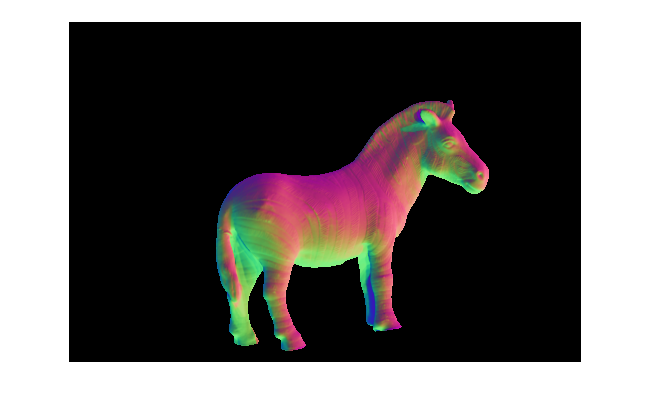
\includegraphics[height=1.2in]{zebraNM}
    \end{subfigure}%
    ~ 
    \begin{subfigure}[]{0.33\textwidth}
        \centering
        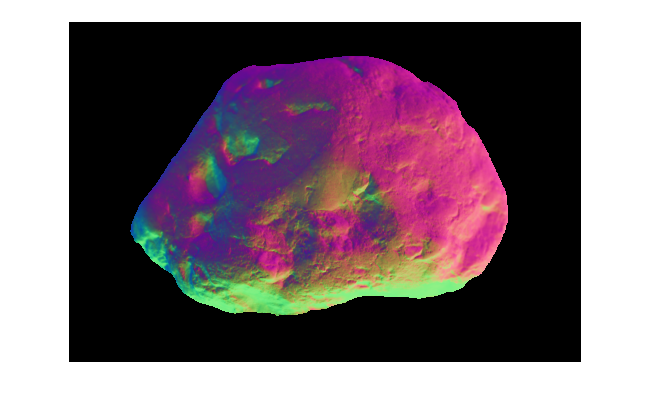
\includegraphics[height=1.2in]{rockNM}
    \end{subfigure}

    \caption{Normal maps}    
\label{fig:NM}

\end{figure*}


\begin{figure*}[h!]
    \centering
    \begin{subfigure}[]{0.33\textwidth}
        \centering
        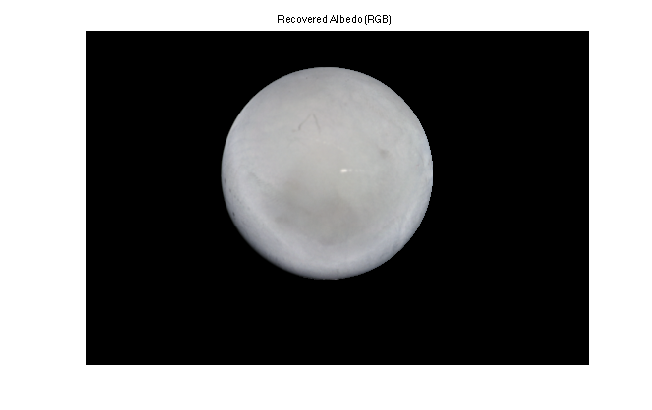
\includegraphics[height=1.2in]{sphereRGB}
    \end{subfigure}%
    ~ 
    \begin{subfigure}[]{0.33\textwidth}
        \centering
        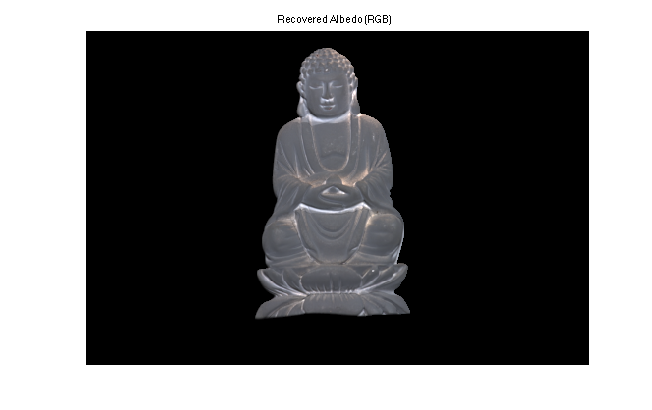
\includegraphics[height=1.2in]{buddhaRGB}
    \end{subfigure}%
    ~ 
    \begin{subfigure}[]{0.33\textwidth}
        \centering
        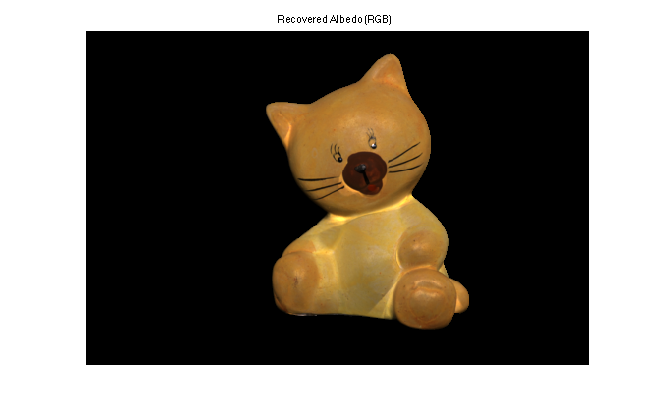
\includegraphics[height=1.2in]{catRGB}
    \end{subfigure}
        \begin{subfigure}[]{0.33\textwidth}
        \centering
        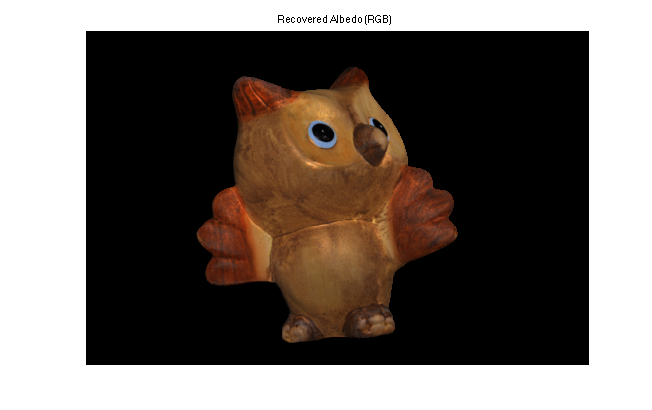
\includegraphics[height=1.2in]{owlRGB}
    \end{subfigure}%
    ~ 
    \begin{subfigure}[]{0.33\textwidth}
        \centering
        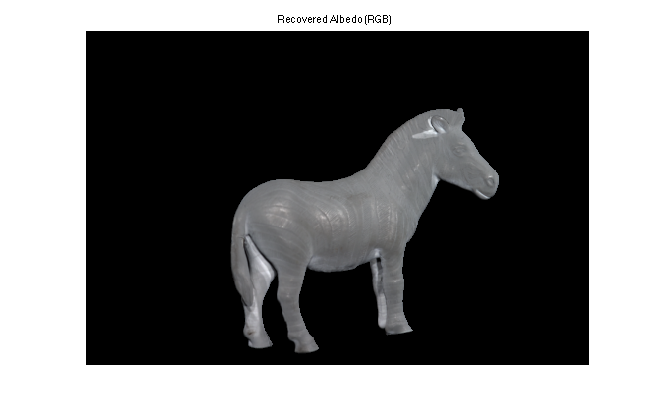
\includegraphics[height=1.2in]{zebraRGB}
    \end{subfigure}%
    ~ 
    \begin{subfigure}[]{0.33\textwidth}
        \centering
        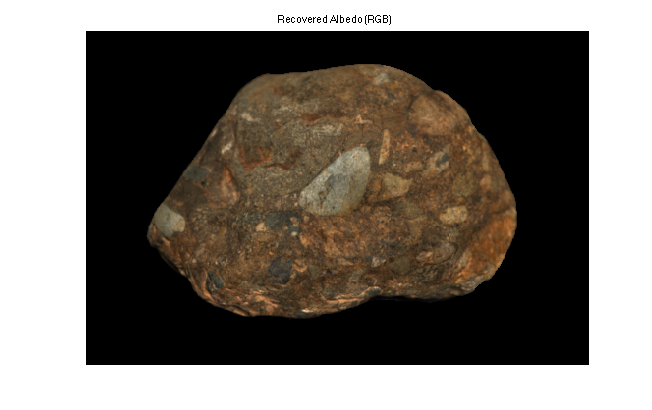
\includegraphics[height=1.2in]{rockRGB}
    \end{subfigure}

    \caption{Recovered RGB albedo}    
\label{fig:RGB}
\end{figure*}

\paragraph{3. Surface Fitting (35 points)}
\subparagraph{Algorithm} 
Let $S(x,y)=(x,y,z(x,y))$ be the surface we would like to recover. The
tangent vectors are then given by 
\begin{equation}
\begin{split}
t_x = \frac{\partial S}{\partial x} = (1, 0, z_x)^T \\
t_y = \frac{\partial S}{\partial y} = (0, 1, z_y)^T
\end{split}
\label{eq:tang}
\end{equation}
where $z_x = \frac{\partial z}{\partial x}$. The estimated normal
$n(x,y)$ should then be consistent with 
\begin{equation}
n(x,y) = \frac{t_x\times t_y}{\Vert t_x\times t_y \Vert} = \frac{(z_x, z_y, -1)^T}{\Vert (z_x, z_y, -1) \Vert}
\end{equation}
Using forward differences to approximate the depth-derivatives, we get
\begin{equation}
\begin{split}
z_x \approx z(x+1,y)-z(x,y) \\
z_y \approx z(x,y+1)-z(x,y)
\end{split}
\label{eq:dz}
\end{equation}
Substituting equation (\ref{eq:dz}) in equation (\ref{eq:tang}) we get an
approximation of the tangent vectors as 
\begin{equation}
\begin{split}
t_x(x,y) \approx (1, 0,  z(x+1,y)-z(x,y) )^T \\
t_y(x,y) \approx  (0, 1, z(x,y+1)-z(x,y))^T
\end{split}
\label{eq:tangAppr}
\end{equation}
We know that these tangent vectors should be perpendicular to the
normal-vector and can therefore introduce the constraints
\begin{equation}
\begin{split}
(1, 0,  z(x+1,y)-z(x,y) ) \cdot n(x,y)=0 \\
 (0, 1, z(x,y+1)-z(x,y))\cdot n(x,y)=0
\end{split}
\end{equation}
Which is equal to:
\begin{equation}
\begin{split}
(z(x+1,y)-z(x,y)) \cdot n_z(x,y)=-n_x(x,y) \\
(z(x,y+1)-z(x,y)) \cdot n_z(x,y)=-n_y(x,y)
\end{split}
\label{eq:const}
\end{equation}
Let $\tilde{z}$ be the vectorization of the $m\times n$ matrix $z$
such that $z(x,y)=\tilde{z}((x-1)n+y)$ and let $\tilde{n}(p)=(\tilde{n}(p)_x,\tilde{n}(p)_y,\tilde{n}(p)_z)$ be
defined similarly. Equation (\ref{eq:const}) can then be rewritten as 
\begin{equation}
A\tilde{z}=b, 
\label{eq:lin}
\end{equation}
where $A$ is an $2mn\times mn$ matrix and $b$ is a vector of length
$mn$. $A$ and $b$ encode equation (\ref{eq:const}) as follows: 

Let $i=(x-1)n+y$ for any position $(x,y)$ on the object. The entries of $A$ are then given by
\begin{equation}
A(2i-1,j) = \begin{cases}
-\tilde{n}_z(i) &\text{if $j=i$}\\
\tilde{n}_z(i) &\text{if $j=i+n$}\\
0 &\text{otherwise}
\end{cases}
\end{equation}
and 
\begin{equation}
A(2i,j) = \begin{cases}
-\tilde{n}_z(i) &\text{if $j=i$}\\
\tilde{n}_z(i) &\text{if $j=i+1$}\\
0 &\text{otherwise}
\end{cases}
\end{equation}

The entries of $b$ can in turn be  computed as:
\begin{equation}
b(k) = \begin{cases}
-\tilde{n}_x(i) &\text{if $k=2i-1$}\\
-\tilde{n}_y(i) &\text{if $k=2i$}\\
0 &\text{otherwise}
\end{cases}
\end{equation}
Note that $A$ is a sparse matrix and the system (\ref{eq:lin}) can
therefore be solved efficiently. The so recovered depth $z$ is then
fixed such that minimum depth is equal to zero. 

Omitted detail: In case points $(x+1,y)$ or $(x,y+1)$ would not belong to the object, backward-differences were used in the derivation of $A$ (adjusting equation (\ref{eq:tangAppr}) accordingly) 

\subparagraph{Results} 
Figure \ref{fig:DM} shows the recovered depth-maps for the six datasets. The
image intensities correspond to the relative depth of the pixels,
where brighter pixels are closer than darker ones.
\begin{figure*}[h!]
    \centering
    \begin{subfigure}[]{0.33\textwidth}
        \centering
        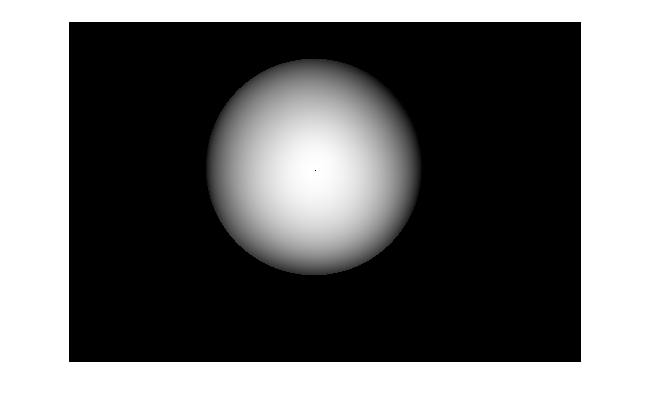
\includegraphics[height=1.2in]{sphereDM}
    \end{subfigure}%
    ~ 
    \begin{subfigure}[]{0.33\textwidth}
        \centering
        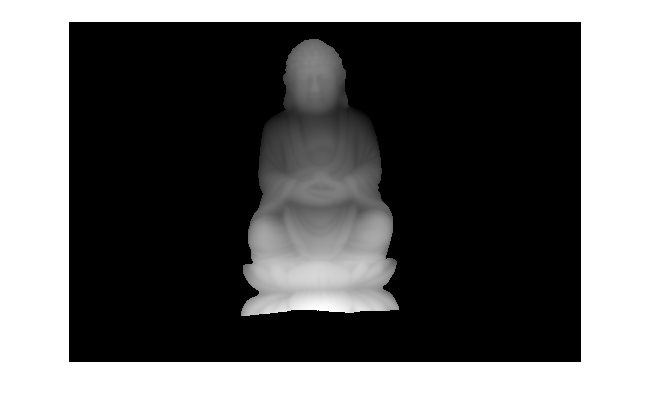
\includegraphics[height=1.2in]{buddhaDM}
    \end{subfigure}%
    ~ 
    \begin{subfigure}[]{0.33\textwidth}
        \centering
        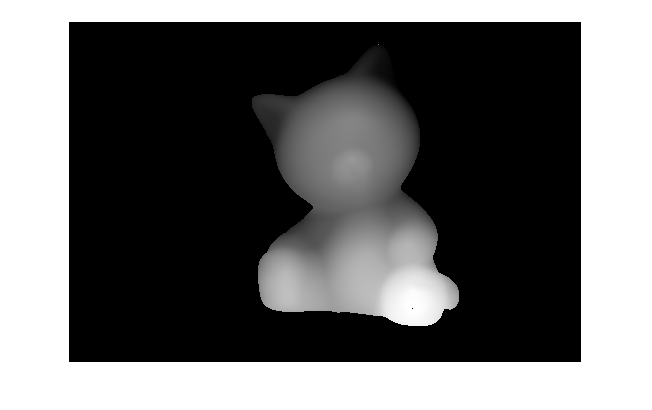
\includegraphics[height=1.2in]{catDM}
    \end{subfigure}
        \begin{subfigure}[]{0.33\textwidth}
        \centering
        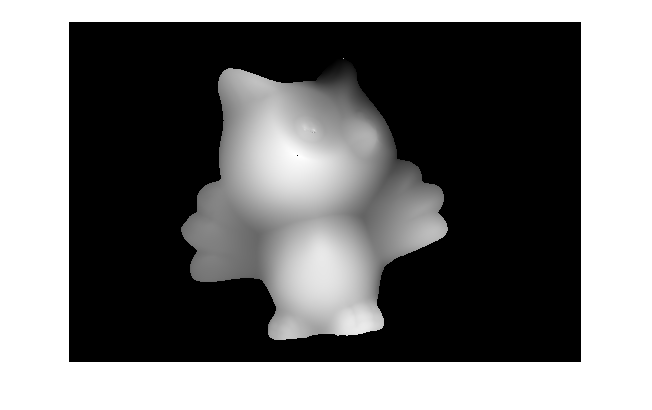
\includegraphics[height=1.2in]{owlDM}
    \end{subfigure}%
    ~ 
    \begin{subfigure}[]{0.33\textwidth}
        \centering
        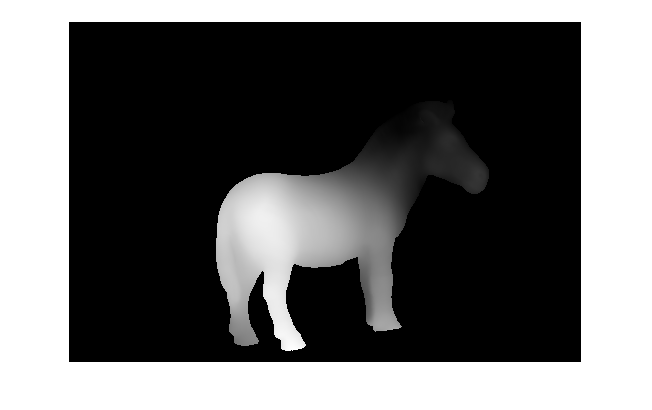
\includegraphics[height=1.2in]{zebraDM}
    \end{subfigure}%
    ~ 
    \begin{subfigure}[]{0.33\textwidth}
        \centering
        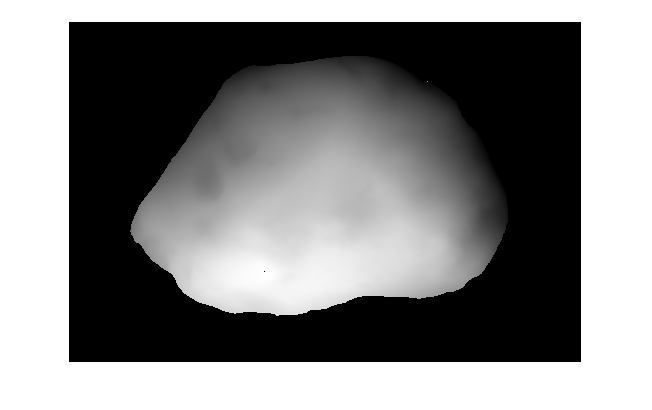
\includegraphics[height=1.2in]{rockDM}
    \end{subfigure}
    \caption{Recovered depth-maps}    
\label{fig:DM}
\end{figure*}

\subparagraph{Discussion} 
It can be observed that sometimes the method can fail in dark regions like the owl's eye, where we can observe a spike in the depth-map. The reason for this is most likely that shading can hardly be observed in dark regions as they barely reflect light. 

Another source of errors, namely shadows, can much better be observed in the recovered albedos and normals. Because the method, as it is presented here, doesn't handle shadowed areas separately, the lower brightness in these areas is "interpreted" as shading by the method, which then leads to wrong results. These effects can be best observed in the neck-region of the buddha and cat, as well as the ear and leg of the zebra. 

Specular reflections, another likely cause of failures, are not clearly observable in the given data and the assumption of Lambertian surfaces seems justified. 

In bright regions with diffuse reflections and without shadows the results of the method are rather convincing. 

 \end{document}